\documentclass[12pt]{article}

\usepackage{graphicx}
\usepackage{titlesec}
\usepackage{xcolor}
\usepackage{enumitem}
\usepackage{subcaption}
\usepackage{float}
\usepackage{placeins}
\usepackage[most]{tcolorbox}
\usepackage[italian]{babel}
\usepackage[a4paper, margin=75pt]{geometry}
\usepackage[colorlinks=true, linkcolor=black]{hyperref}

\graphicspath{{images/}}
\setlist{itemsep=2pt}
\definecolor{greenpastel}{RGB}{180, 230, 180}
\tcbset{
  myboxstyle/.style={
    colback=white,
    coltitle=black,
    fonttitle=\bfseries,
    boxrule=1pt,
    rounded corners,
    enhanced,
    attach boxed title to top left={xshift=5mm},
    boxed title style={
        size=fbox,
        colback=greenpastel,
        boxrule=0pt,
        sharp corners,
        enhanced,
        frame code={
            % Disegno trapezio con base superiore più stretta
            \path[fill=greenpastel, rounded corners=1mm]
                ([xshift=0mm]frame.north west) -- 
                ([xshift=-1mm]frame.north east) -- 
                ([xshift=2mm]frame.south east) -- 
                ([xshift=-3mm]frame.south west) -- cycle;
        },
        interior hidden
    }
  }
}

\newcounter{definition}[section]
\renewcommand{\thedefinition}{
  \thesection
  \ifnum\value{subsection}>0 .\arabic{subsection}\fi
  \ifnum\value{subsubsection}>0 .\arabic{subsubsection}\fi
  .\arabic{definition}
}
\newtcolorbox{definition}[1][]{
  myboxstyle,
  colframe=greenpastel,
  boxed title style={colback=greenpastel},
  before title={\refstepcounter{definition}},
  title={Definizione \thedefinition: #1}
}


\titleformat{\section}
  [block]
  {\raggedleft\LARGE\bfseries}
  {\textcolor{gray}{\scalebox{5}{\thesection}}}
  {0pt}
  {\\[3pt]}

\titlespacing*{\section}
  {0pt}   % rientro sinistro
  {0pt}   % spazio prima della sezione
  {30pt}  % spazio dopo la sezione

\begin{document}
    % --- Copertina ---
    \begin{titlepage}
        \centering

        % --- Logo Sapienza ---
        
\includegraphics[width=0.95\textwidth]{logo_sapienza.png}
        
        \vspace*{\stretch{0.2}}
        
        % --- Dati Sapienza ---
        {\LARGE "Sapienza" Università di Roma}\\[3pt]
        {\Large Ingegneria dell'Informazione, Informatica e Statistica}\\[3pt]
        {\large Dipartimento di Informatica}\\[3pt]
        
        % --- Spazio vuoto ---
        \vspace*{\stretch{1}}
        
        % --- Titolo ---
        \hrulefill\\
        \vspace{15pt}
        \textbf{\huge Programmazione WEB}\\
        \vspace{7pt}
        \hrulefill\\
        
        % --- Spazio vuoto ---
        \vspace*{\stretch{2}}
        
        % --- Autore ---
        \textit{\Large Autore}\\[3pt]
        {\Large Vincenzo Bova}\\
        
        % --- Spazio vuoto ---
        \vspace*{\stretch{1}}

        % --- Data ---
        {\large A.A. 2025/2026}\\
    \end{titlepage}

    % --- Indice ---
    \newpage
    \tableofcontents

    % --- Introduzione a Git ---
    \newpage
    \section{Introduzione a Git}
    \subsection{Sistemi di versionamento}
    Durante lo sviluppo di un progetto c'è spesso la necessità di effettuare revisioni, correzioni o modifiche ai file che lo compongono.
    \begin{figure}[H]
        \centering
        
\includegraphics[width=0.5\textwidth]{introduzione_a_git/no_git_example.png}
    \end{figure}
    Gestire ciò creando ogni volta nuovi file, tuttavia, comporta evidenti problemi:
    \begin{itemize}
      \item \textbf{Duplicazione del contenuto:} che rende il sistema inefficiente e aumenta la difficoltà nel mantenere integrità;
      \item \textbf{Assenza di Naming Convention:} che rende impossibile risalire ad uno storico delle modifiche;
      \item \textbf{Autori incerti};
      \item ...
    \end{itemize}
    \begin{samepage}
      Per ovviare a ciò sono stati creati i \textbf{sistemi di versionamento} (git, csv, mercurial, svn...), i quali offrono vari benefici:
      \begin{itemize}
        \item \textbf{Gestione delle versioni:} il sistema si occupa automaticamente di etichettare le varie versioni in modo consistente;
        \item \textbf{Tracciamento delle mofiche:} è possibile accedere ad uno storico delle modifiche effettuate;
        \item \textbf{Presenza di metadati:} ogni modifica ha un autore, una data...;
        \item \textbf{Creazione di linee di sviluppo parallele:} è possibile creare una versione parallela del codice per non modificare la versione principale, e poi riunirle integrando i cambiamenti;
        \item \textbf{Sincronizzazione tra computer:} il sistema consente di mantenere il progetto allineato tra più computer.
      \end{itemize}
    \end{samepage}

    \subsection{Git}
    Git è un sistema di versionamento distribuito e veloce, creato nel 2005 e capace di gestire progetti di grandi dimensioni.
    Si basa su un design semplice e utilizza DAG (\textit{Directed Acyclic Graph}) e Merkle trees come strutture dati.
    \begin{definition}[Repository]
      È un insieme di commit, branch e tag.\\
      Per semplicità assumiamo che un progetto equivale ad un repository.
    \end{definition}
    \begin{definition}[Working copy]
      È un insieme di file tracciati nella copia locale.\\
      Un nuovo file non sarà ancora tracciato e bisognerà aggiungerlo.\\
      Quando aggiorniamo i file (\textit{update}), stiamo aggiornando la working copy.
    \end{definition}
    
    \subsubsection{Commit}
    Un commit è un'istantanea del repository in un determinato momento.\\
    Viene identificato dallo \textbf{SHA1} del commit stesso e contiene diversi campi:
    \begin{itemize}
      \item data + autore, data + commiter
      \item commento \textbf{obbligatorio}
      \item 0,1 o più genitori
      \item tree: hash di tutti i file nel commit
    \end{itemize}
    \begin{minipage}{\textwidth}
      In particolare il commit può contenere un sottoinsieme delle modifiche (anche ad un singolo file), le quali devono essere aggiunte alla staging area dei cambiamenti.
      \begin{figure}[H]
        \centering
        \begin{subfigure}{0.49\textwidth}
          \centering
          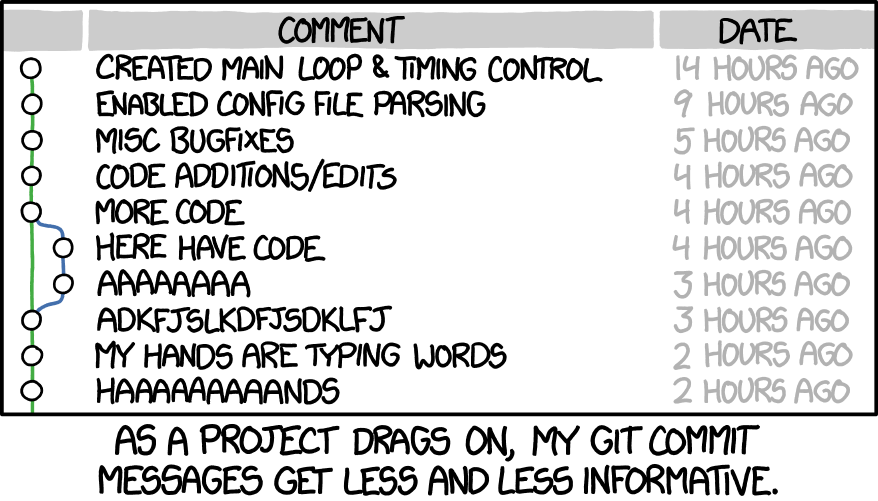
\includegraphics[height=4cm]{introduzione_a_git/git_commit.png}
        \end{subfigure}
        \hfill
        \begin{subfigure}{0.49\textwidth}
          \centering
          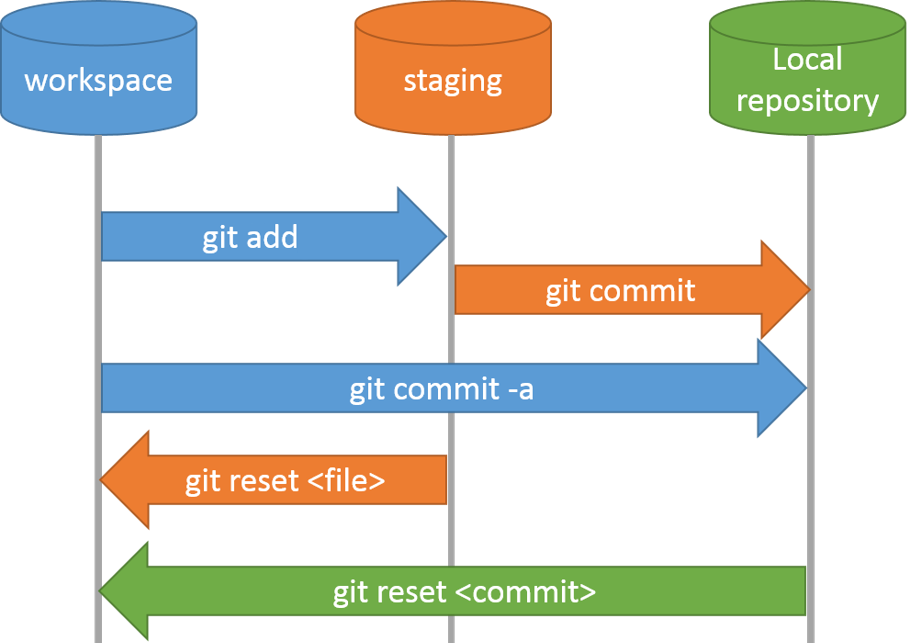
\includegraphics[height=4cm]{introduzione_a_git/git_commit_staging.png}
        \end{subfigure}
      \end{figure}
    \end{minipage}

    \subsubsection{Branch}
    Un branch è una linea di sviluppo, composta da un insieme ordinato di commit collegati in un DAG, il quale inizia dal primo commit del repository e punta all'ultimo commit.\\
    Grazie ai branch è possibile \textbf{lavorare parallelamente} a più versioni del progetto.
    \begin{figure}[H]
      \centering
      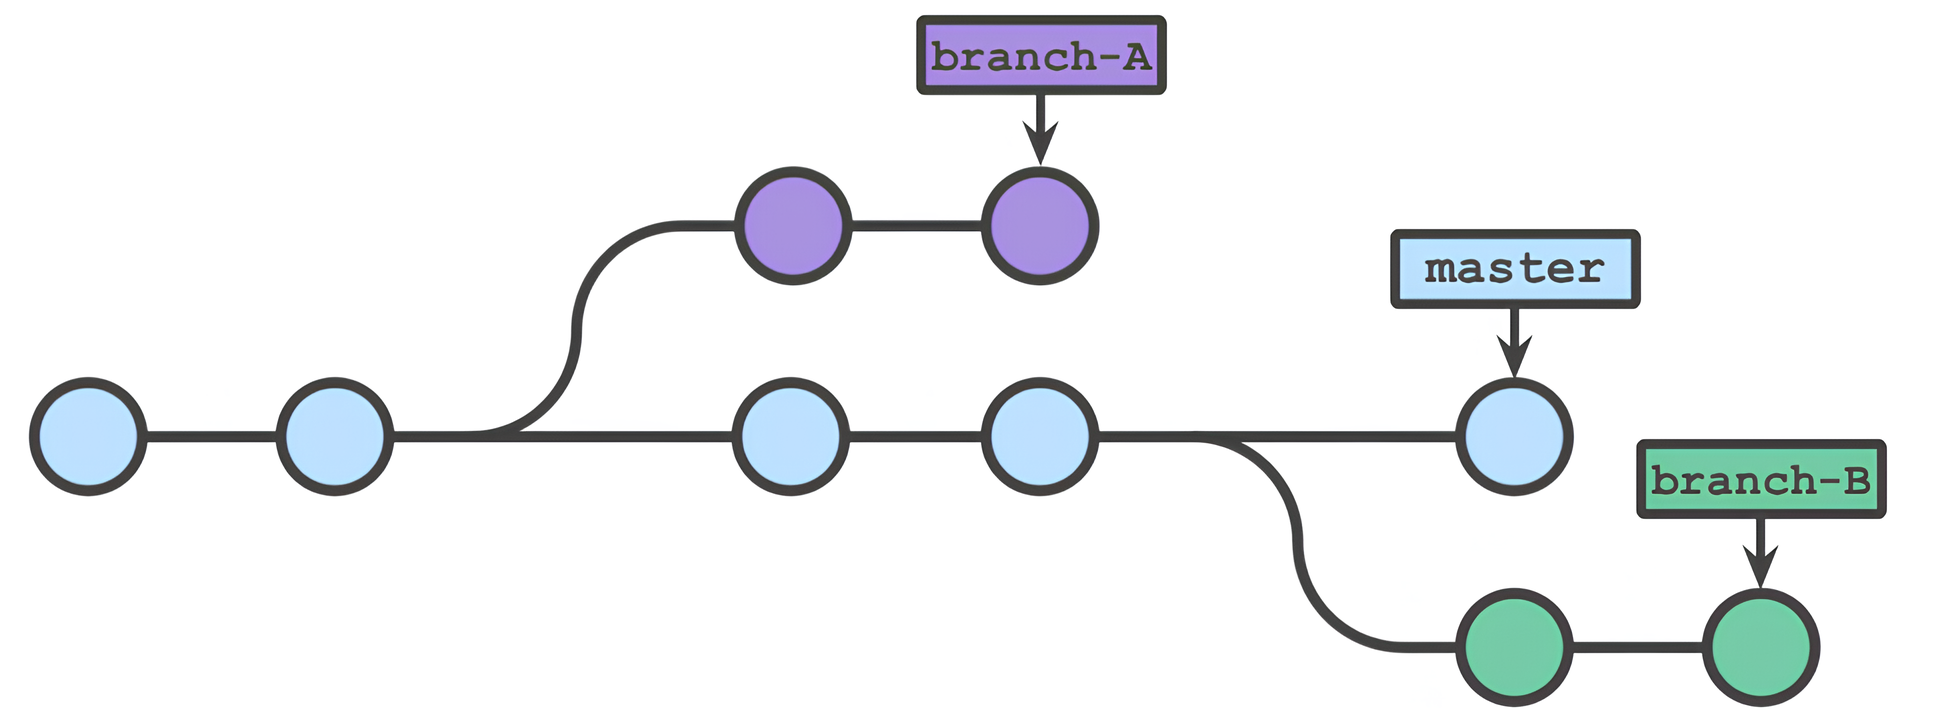
\includegraphics[width=0.7\textwidth]{introduzione_a_git/branch.png}
    \end{figure}

    \subsubsection{HEAD}
    L'HEAD è un puntatore alla posizione attuale rispetto alla storia del repository e può essere aggiornato tramite il comando \textit{checkout}.\\
    Solitamente l'HEAD punta ad un branch o ad un tag, qualora invece puntasse ad un commit si parlerebbe di \textbf{Detached HEAD}. Quando ci si trova in questo stato i commit fatti non vengono inseriti in alcun branch, rischiando quindi di andare persi.
    \begin{figure}[H]
      \centering
      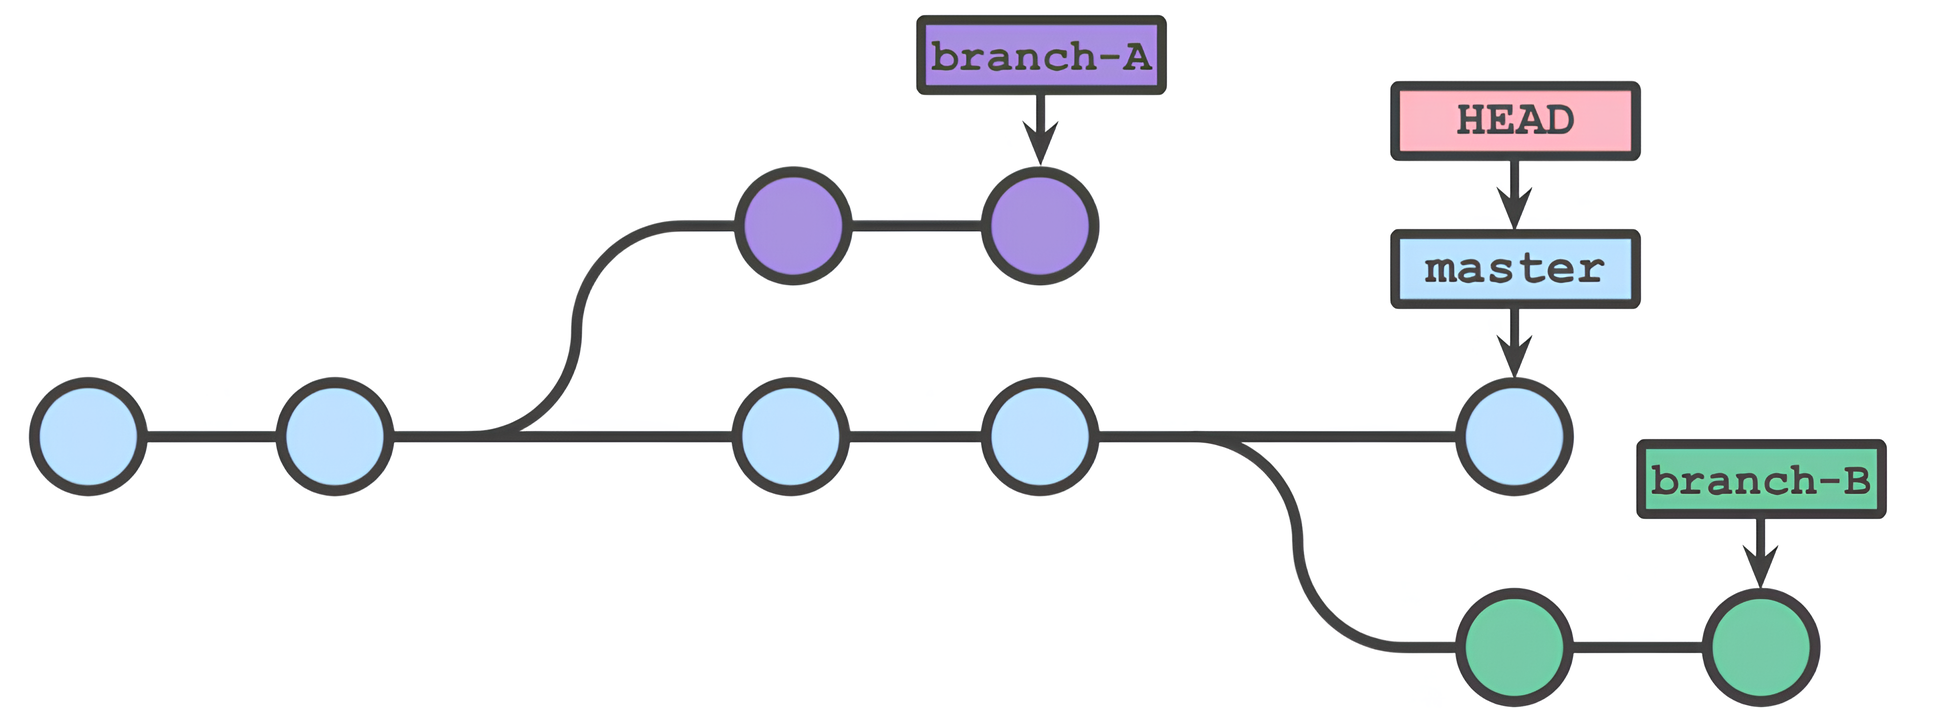
\includegraphics[width=0.7\textwidth]{introduzione_a_git/branch_head.png}
    \end{figure}

    \subsubsection{Tag}
    Un tag è un'etichetta per un commit e viene solitamente usato per segnare versioni importandi di un progetto (e.g. \textit{v1.0.0}, \textit{release-2025-09}).

    \subsubsection{Merge}
    Il merge è un'operazione che fonde i cambiamenti tra due branch, facendo in modo che la destinazione contenga entrambi i cambiamenti mentre l'origine rimanga immutata.\\
    Può avvenire mediante tre strategie:
    \begin{itemize}
      \item \textbf{Fast forward:} quando il branch di destinazione non ha commit successivi rispetto a quello che si vuole unire e il sistema sposta semplicemente il puntatore in avanti;
      \item \textbf{Merge commit:} quando i branch hanno sviluppi indipendenti e il sistema crea un nuovo commit con due genitori;
      \item \textbf{Rebase:} il sistema ricrea ogni commit non in comune tra i due branch, mantendo così una storia lineare.
    \end{itemize}
  
    \subsection{Comandi Git}
    
\end{document}
